\documentclass[a4paper]{article}
\usepackage{graphicx}
\usepackage{epstopdf}
\usepackage{mcode}
\usepackage{float}
\title{Laboration i Komponentfysik\\ Optoelektronik}

\author{Alexander Najafi \\ Linus Hellman}

\date{2014-04-13}

\begin{document}

\maketitle
\thispagestyle{empty}
\newpage

\tableofcontents
\newpage

\section{Inledning och bakgrund}

Denna lab är utformad för att ge en större förståelse för halvledarkomponenter och dess samverkan med ljus, både emission (ljusluminicens) samt absorption kommer undersökas. Detta har ett extremt stort användningsområde tillexempel i kameror, där ljus ska översättas till digital data. Under labben kommer det kontrolleras om det stämmer att den våglängd som stämmer överens med bandgapsenerginkommer att lysa med störst intensitet. Vidare kommer också absorptionskurvan att studeras. Teorin säger att fotodioden kommer börja absorbera fotoner i rymdladdningsområdet först då fotonerna har en våglängd som ger en energi som är lika med eller större än bandgapsenergin enligt $\lambda = hc/E_{fot}$, men då rymdladdningsområdet ligger en bit under ytan kommer absorptionskonstanten att öka i takt med fotonenergin och det leder till att absorptionen kommer minska igen enligt följande formel.

\begin{equation}
  \Phi(x) =\Phi_0e^{-\alpha x}
\end{equation}

Diodens uppbyggnad kommer även studeras då en egen diod kommer tillverkas och analyseras. Denna kommer konstrueras med hjälp av en platta av Galliumfosfid som kommer legeras med dels tenn dels zinklegerat guld. Detta kommer att n-,p-dopa GaP-biten tillräckligt för att den ska få en diods egenskaper. 

Vidare kommer en analys göras på en solcell för att undersöka vid vilken belastningsresistans denna uppnår sin maximala effekt. Belysning av en diod kommer att leda till en ström genom dioden. Men om ingen belastningsresistans finns kommer det inte ligga någon spänning över dioden alltså ingen effekt. Om det istället ligger oändligt mycet belastning över dioden kommer det inte att gå någon ström, alltså ingen effekt. Det som måste göras är att hitta den punkt i ström/spänningkurvan som ger den största arean ($U*I=effekten$).
\newpage
\section{Resultat}
\subsection{Dioden}
Dioden som tillverkades hade en framspänning på 0.6V och en backspänning på 3.4V. I figur \ref{diodiv} synes I-V-kurvan som togs fram på labben med oscilloskopet.
\begin{figure}[H]
	\centering
	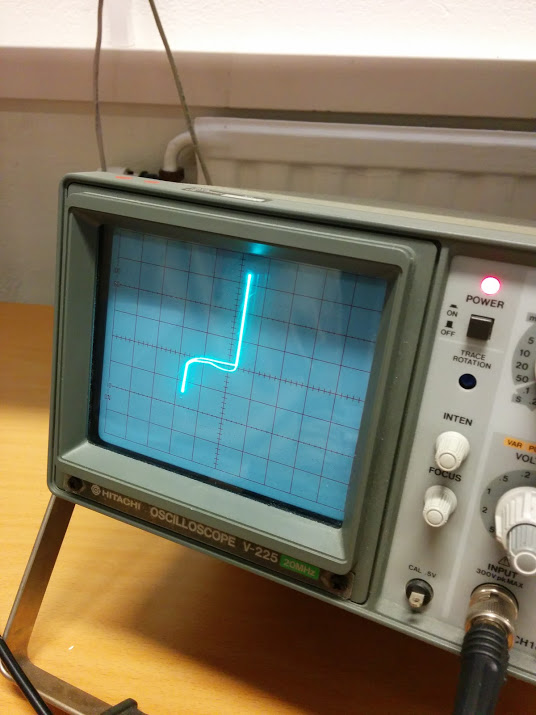
\includegraphics[scale=.4]{diod.jpg}
	\caption{I-V-kurva som syns på oscilloskopet}
	\label{diodiv}
\end{figure}
\subsection{Solcellen}
Följande I-V-kurva togs fram för solcellen. För matlab-kod och data se bilaga.
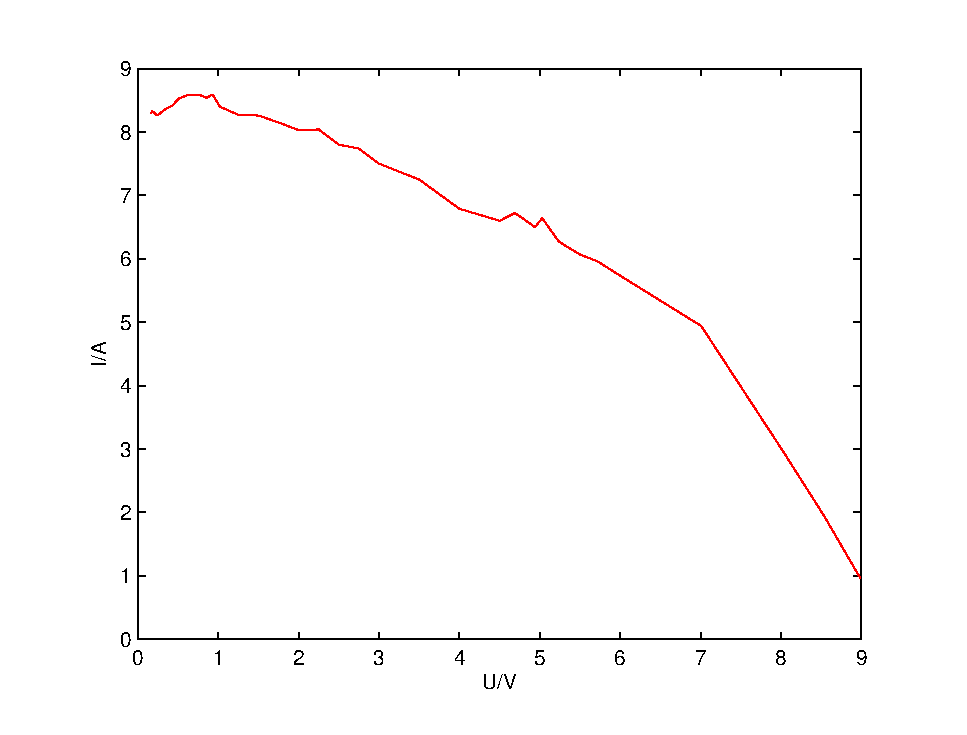
\includegraphics[scale=.7]{solcell.eps}
\newpage
\appendix
\section{Matlabkod}
\subsection{Solcellen}
\lstinputlisting{solcell.m}
\end{document}
